\chapter{Spectroscopy and the {\it K}-band Multi-Object Spectrograph}
\label{ch:kmos}
\renewcommand{\headrulewidth}{1pt}
\fancyhead[RO]{\textit{Chapter \thechapter: Spectroscopy and KMOS}}
\fancyhead[LE]{\textit{Red Supergiant Stars in the Local Group and Beyond}}

\section{Opening Remarks} % (fold)
\label{sec:opening_remarks}
This chapter initially describes the basic design of a spectrograph and outlines some of the more commonly used spectroscopic techniques, in Section~\ref{sec:intro_to_spec}.
I then describe integral field spectroscopy, a more complex spectroscopic technique, in Section~\ref{sec:IFS}, which leads to Section~\ref{sec:KMOS}, where I describe KMOS and, in Section~\ref{sec:3Ddata} the KMOS data  and data reduction process is outlined.
Finally, I conclude the chapter in Section~\ref{sec:kmosconc}.

KMOS warrants an individual chapter in this thesis as all of the spectroscopic observations presented in the proceeding chapters are observed this instrument.

% section opening_remarks (end)

\section{Introduction to Spectroscopic Techniques} % (fold)
\label{sec:intro_to_spec}

Spectroscopy is the study of the dispersion of light into its constituents and has been at the forefront of astronomy for roughly the last 200 years.
Sir Isaac Newton demonstrated the principles of spectroscopy (and coined the term ``spectrum'') using light from The Sun in his seminal ``Opticks'' work~\citep{b:Newton}.
By using the groove spacings on a diffraction grating, Thomas Young first quantified the wavelengths of different colours of light~\citep{1802PTRSL.92.12Y}.
The simple set-up of a spectrograph, which has -- more or less -- been used since the early spectroscopic experiments, consists of five basic elements:

\begin{enumerate}
    \item slit,
    \item collimator,
    \item dispersive element,
    \item camera and
    \item detector.
\end{enumerate}

A simple spectrograph is illustrated in Figure~\ref{fig:spectrograph}.
In Newton's demonstration a small hole in the window blinds was used as a slit, and a screen as a detector.
The slit in modern spectroscopic observations can take various forms.
Today, the most widely used type of spectoscopic observation is long-slit spectroscopy.
Using a long slit, a spectrum is taken for each spatial pixel along the length of the slit.
This is demonstrated in Figure~\ref{fig:long-slit}, where the final panel shows that each pixel illuminated within the slit produces a spectrum.
This can be thought of a 2-dimensional spectroscopy, which is particularly useful when attempting to take a spectrum of an extended object
(rather than a point source).

\begin{figure}
 \centering
 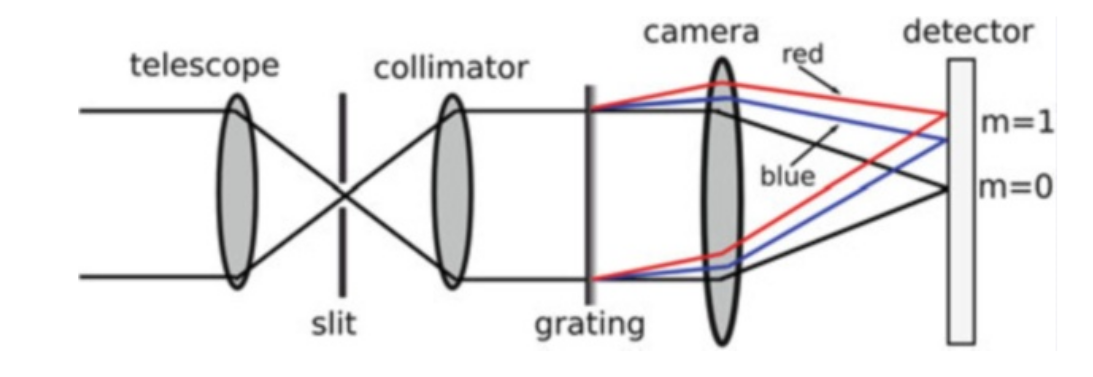
\includegraphics[width=0.65\textwidth]{kmos/Lawrence-spectrograph}
 \caption[A simple spectrograph]{A simple spectrograph detailing the five basic elements of a simple spectrograph: slit, collimator, dispersive element, camera and detector.
 Credit:~\cite{2014amcg.book.....L}.
 \label{fig:spectrograph}}
\end{figure}

\begin{figure}
 \centering
 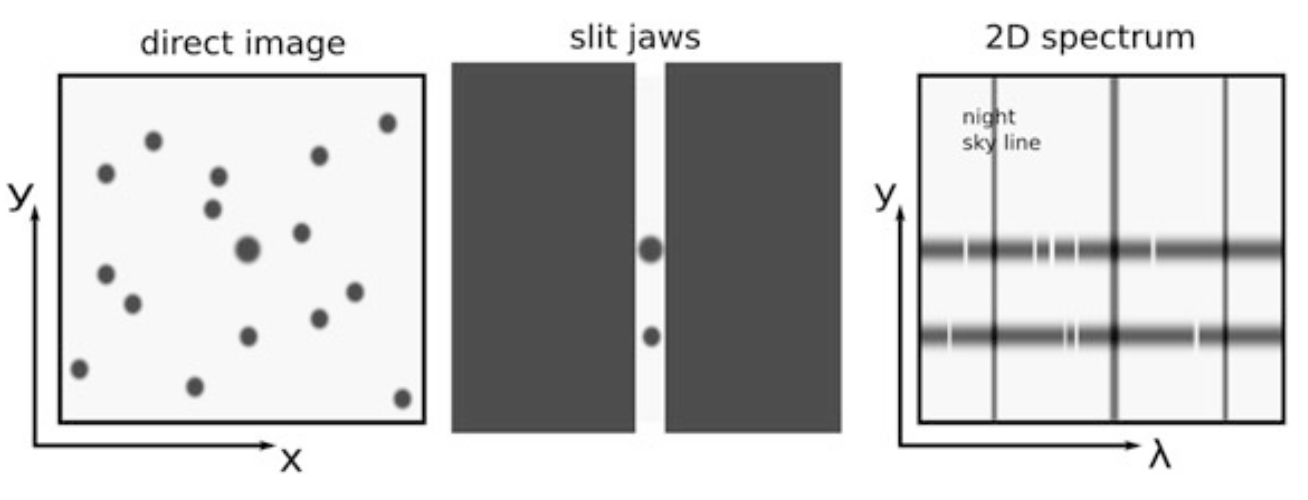
\includegraphics[width=0.65\textwidth]{kmos/Lawrence-long-slit}
 \caption[Long-slit spectroscopy]{Three panels demonstrating long-slit spectroscopy.
 The left panel shows what an image of the field-of-view.
 The central panel illustrates that the long slit selects only the slit width in the $x$-axis and the full $y$-axis range.
 The right panel shows that for each pixel in the $y$ direction, a spectrum is obtained.
 Credit:~\cite{2014amcg.book.....L}.
 \label{fig:long-slit}}
\end{figure}

An alternative to using a long-slit to remove contamination from other sources is to use a small hole or fibre to select the target flux.
By precisely drilling a hole in a metal plate, a slit is created that can be used to select the target flux.
One of the advantages of using this method is that more than one object can be selected for a single exposure.
By creating multiple slits within a single plate, spectroscopy of multiple objects can be obtained where contamination from other sources is minimised.
This method was improved on by introducing optical-fibres positioned within the holes.
Figure~\ref{fig:multi-obj} details the principles of multi-object spectroscopy using optical-fibres.
The fibres could then be led to an instrument that was not directly attached to the telescope, which has the advantage that the instrument will not suffer from the changing gravitational force as the telescope moves.
In addition, the conditions within the instrument room can be controlled.
This is particularly important for near-IR spectrographs and detectors, where thermal radiation is particularly important to minimise.

However, using a plate with several holes has some drawbacks.
These include, the time taken to create the slit mask, the lack of flexibility while observing and the operational costs of creating a new mask each time a different field is to be observed~\citep{1986SPIE..627..118P}.
These reasons, in addition to improved computing power, led to the development of instruments that were able to automatically position fibres~\citep{1982SPIE..331..289T}.
Most modern fibre-fed spectrographs have automatic fibre-positioning technology which is broadly split up into two approaches:

\begin{enumerate}
    \item Each fibre has a magnetic button attached and a single robot is charged with moving each fibre sequentially.
    This is an effective method to place large numbers of fibres, but does however, take a significant length of time for each configuration.
    \item Each fibre is mounted upon a computer-controlled arm.
    This method is generally less time consuming but increases the instrument build cost.
\end{enumerate}

As a variant on the five basic elements of a spectrograph, slitless spectroscopy is also a feasible option, which is not discussed in detail here.
For a thorough overview on slitless spectroscopy see~\citet{2014PhDT.........C}.

\begin{figure}
 \centering
 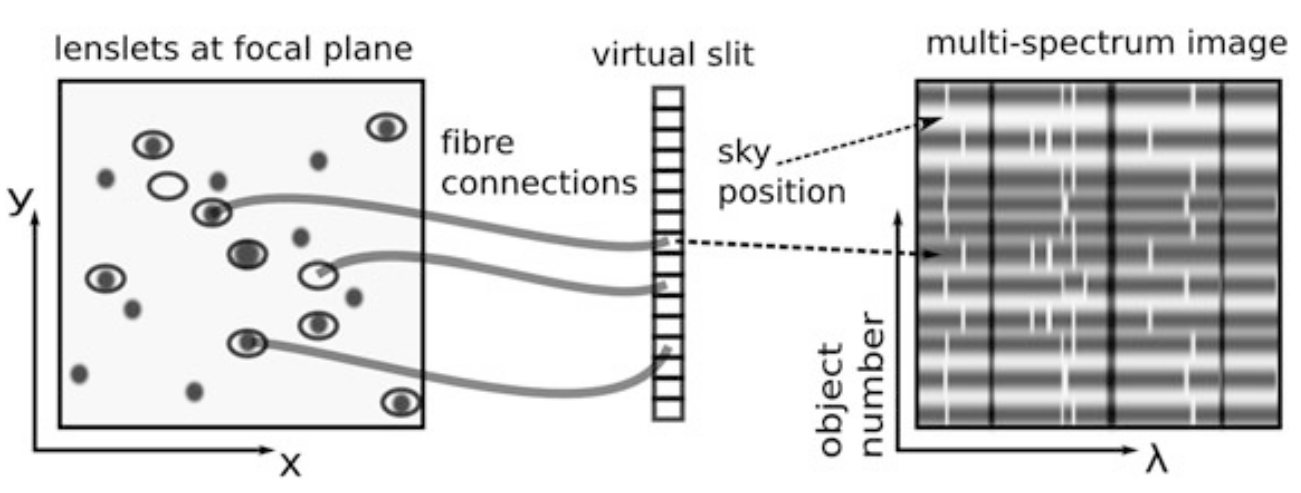
\includegraphics[width=0.65\textwidth]{kmos/Lawrence-multi-object}
 \caption[Multi-object spectroscopy]{Three panels demonstrating multi-object spectroscopy.
 The left panel shows what an image of the field of view.
 The central panel illustrates that each fibre in this simple multi-object spectrograph can be positioned at any point throughout the field of view and is rearranged into a pseudoslit.
 The right panel shows that for each pixel in the $y$ direction, a spectrum is obtained.
 Credit:~\cite{2014amcg.book.....L}.
 \label{fig:multi-obj}}
\end{figure}

A key element to any spectrograph is the dispersive element.
In Newton's original experiments this took the form of a glass triangular prism.
A prism disperses light based on the wavelength dependence of the refractive index of glass: differential refraction.
This produces a low-resolution spectrum spanning a large spectral range.

Typically in modern spectrographs the dispersive element is a diffraction grating.
A diffraction grating consists of a reflective surface with many parallel grooves.
These grooves act as slits and disperse the light which is then combined on the detector through the interference of light using the same principles as a double slit experiment.
Figure~\ref{fig:doubleslit} shows a sketch of the interference pattern, from Young's original experiment, for monochromatic light striking two slits of width $a$, with separation $d$, at wavelength $\lambda$.
By increasing the number of slits the fringe maxima remain stationary while becoming narrower and more intense.
The angular positions ($\theta$) of the fringe maxima are,


\begin{figure}
 \centering
 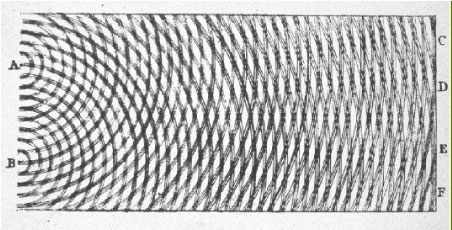
\includegraphics[width=0.65\textwidth]{kmos/youngslits}
 \caption[Double slit interference pattern]{A double slit interference pattern from Thomas Young's original experiments.
 \label{fig:doubleslit}}
\end{figure}


\begin{equation}
    sin\,\theta = \frac{m\lambda}{d},\label{eq:a}
\end{equation}

\noindent where $m$ is an integer and refers to the fringe order ($m$~=~0 for the central undispersed peak).
As the number of secondary peaks depends upon the number of rulings $N$, the angular positions of the zero positions also depend upon $N$,

\begin{equation}
    sin\,\theta = \frac{m'\lambda}{Nd}.\label{eq:b}
\end{equation}

\noindent Therefore, the angular width of the principle maximum between the first two zero positions ($\Delta\theta$ or $W$) is obtained by defining,
\begin{equation}
     W = \Delta m'\frac{d\theta}{dm'},\label{eq:c}
\end{equation}

\noindent and by differentiating equation~\ref{eq:b},

\begin{equation}
    W = \frac{2\lambda}{Nd\,cos\,\theta}.\label{eq:d}
\end{equation}

\noindent The Rayleigh Criterion states: ``Two point sources are regarded as just resolved when the principal diffraction maximum of one image coincides with the first minimum of the other''~\citep{1880MNRAS..40..254R}.
By the application of this criterion one can define the spectral resolution in terms of the angular separation as,

\begin{equation}
    W = \frac{\lambda}{Nd\,cos\,\theta}.\label{eq:e}
\end{equation}

\noindent which does not depend upon the fringe order.
Typically, the spectral resolution is quoted in terms of the smallest wavelength which can be separated in the spectrum.
This is given by converting the angular width into the corresponding wavelength width using $\Delta\lambda = \Delta\theta\,d\lambda/d\theta$ which gives,

\begin{equation}
    \Delta\lambda = \frac{\lambda}{Nm},\label{eq:f}
\end{equation}

\noindent more commonly quoted as the ratio of the operating wavelength to the spectral resolution,

\begin{equation}
    R = \frac{\lambda}{\Delta\lambda} = Nm,\label{eq:g}
\end{equation}

\noindent where $R$ is the spectral resolving power (or often incorrectly, the resolution).

Separation of the spectral orders is an important consideration in diffraction grating spectroscopy, which can be taken into account by using a broadband blocking filter to limit the spectral range to a single order only.
In principle, higher spectral resolving power can be obtained by viewing higher spectral orders, however, both the intensity of the spectra and spectral range are diminished.
Typically low spectral orders are used in astrophysical observations.

Diffraction gratings have many intrinsic advantages over glass prisms, when used for quantitative spectroscopy, and are generally preferred.
However, they are used in tandem for some applications.
For example, Echelle spectrographs. working in higher orders to achieve higher resolving power, make use of an additional dispersive element, which is often a prism, to spatially separate different orders so that they can be simultaneously recorded on the detector.


Even though prisms are used rarely in modern astronomical spectroscopy they still have some important applications.
The upcoming near infrared spectrograph (NIRSpec) instrument, on the James Webb Space Telescope (JWST), will contain a prism (in addition to several diffraction gratings) to obtain low-resolution spectroscopy of a very large spectral range (0.6--5.3\,$\mu$m).

% section introduction_to_spectroscopic_techniques (end)

\section{Integral Field Spectroscopy} % (fold)
\label{sec:IFS}

The overall goal of integral field spectroscopy (IFS) is to obtain a spectrum of everything (targets and their surroundings) within a given field-of-view (FoV).
This concept builds on the idea that a long-slit spectrograph obtains spectra for targets within the extent of the slit.
A natural extension of this technique would be to use a long-slit spectrograph to obtain a spectrum for each pixel within a 2-D FoV on the sky.

There are many intrinsic advantages to having a specifically designed instrument to perform this task rather than simply repeating observations with a long-slit spectrograph.
These advantages include,

\begin{enumerate}
    \item eliminating slit-losses,
    \item accurate target acquisition is not required,
    \item the target position can be recovered from data,
    \item reduced radial velocity errors from positional issues in the slit when comparing target and reference object,
    \item the velocity field is recovered without biases.
    % \item IFS always optimally samples object point spread function (PSF).
\end{enumerate}

In addition, potentially the most compelling argument is that to perform IFS with a long-slit spectrograph one is required to take $N$ exposures all of length $t_{exp}$, however, using IFS, a spectrum for each spaxel is obtained with a single exposure. Therefore efficiency on-sky is increased.


\subsection{Techniques of integral field spectroscopy} % (fold)
\label{sub:techniques_of_integral_field_spectroscopy}

IFS may be achieved using a variety of different and novel methods.
Potentially, the simplest of these is (and most cost effective in the short term) is to take multiple exposures using an existing spectrograph over a small FoV.
Another, conceptually simple, approach is to take photometric data of the same field using multiple narrow-band filters which can be stitched together to create effectively low-resolution spectra of a FoV~\citep[e.g. GTC-OSIRIS][]{2011PASP..123.1107M}.


There are three main techniques which are more commonly used to generate spectra over a 2-dimensional FoV.
The difference between the techniques is in the way in which they split up the image.
A spectrograph specialised for IFS adds an additional element to the five basic elements of a spectrograph outlined previously: an integral field unit (IFU).
An IFU splits up the image obtained by the telescope into elements, or slices, that are constructed into a slit and dispersed by the dispersive element.
In this section I will detail each of these techniques in turn and conclude by providing a comparison between them.

A lenslet array splits the input image using a tight array of small lenses~\citep{1995A&AS..113..347B}.
The lenses then focus the light of each sub-field separately which are then dispersed.
This technique limits the length of the spectrum measured on the detector.
To improve this, the spectra are tilted about the optical axis to minimise overlapping of spectra, which leads to inefficient packing of the resulting spectra on the detector.
The top row of Figure~\ref{sec:IFS} illustrates IFS using a lenslet array to split the image.


Fibre arrays use a tightly packed bundle of fibre-optic cables to split the telescope image.
The fibres then reposition the image onto a linear slit.
The middle row of Figure~\ref{fig:IFS} illustrates this process.
As the fibre cables are intrinsically cylindrical objects, light is lost between fibres in the focal plane.
To minimise the light lost, this technique can be improved upon by using an array of lenses, to focus the light from each element into the fibre, effectively combining this technique with the previous method.

The final technique is to use an image slicer to split the image from the telescope~\citep{1997SPIE.2871.1295C}.
Figure~\ref{fig:image_slicer} shows an image slicer used in the KMOS instrument.
An image slicer is a type of segmented mirror where each linear segment reflects light in a slightly different direction.
A second segmented mirror then arranges the images into a pseudoslit where it is then dispersed.
As~\cite{2006NewAR..50..244A} demonstrated, this method is intrinsically efficient as complete slices of the field are imaged by the detector.
In addition, this method is also particularly applicable for IR studies as the optical system consists mainly of mirrors which are easily cooled to low temperatures.
Drawbacks with this technique include that a large and complex optical system is required with a surface roughness ($\sigma$) of $\sigma \leq$~10\,nm in the IR.

\begin{figure}
 \centering
 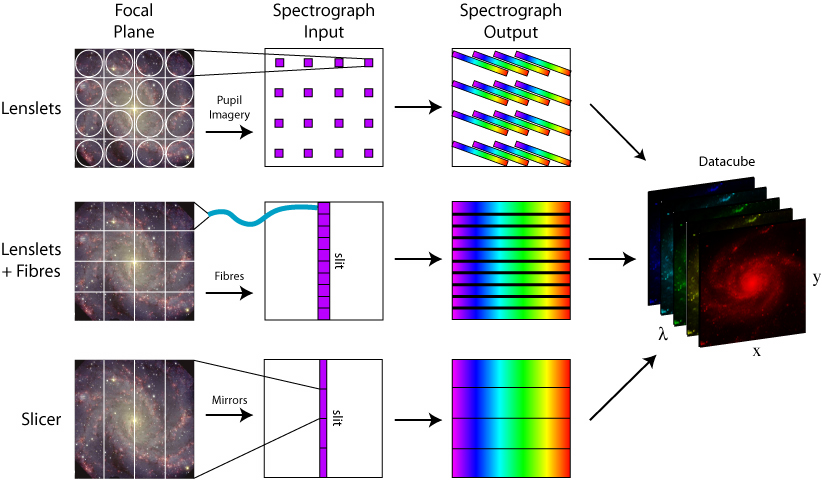
\includegraphics[width=\textwidth]{kmos/ifu_designs}
 \caption[Integral field spectroscopic methods]{Three diagrams demonstrating the techniques of integral field spectroscopy.
 The top row shows how an array of lenslets can be used to focus the light for the spectrograph. The right-hand panel of this row demonstrates that this leads to inefficient packing of the spectra on the detector.
 The middle row shows how a combination of fibres and lenslets can be used to reconstruct a slit and make more efficient use of the detector.
 The bottom panel shows that an image slicer efficiently splits up the field-of-view and reconstructs the slit using mirrors.
 Each technique results in a three-dimensional data cube consisting of $x$, $y$ and $\lambda$ information for each pixel on the detector.
 Credit: M. Westmoquette, adapted from~\citep{2006NewAR..50..244A}.
 \label{fig:IFS}}
\end{figure}

\begin{figure}
 \centering
 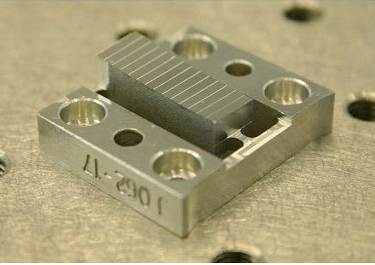
\includegraphics[width=0.65\textwidth]{kmos/kmos-image-slicer}
 \caption[A KMOS image slicer]{An image slicer from one of the arms used in the KMOS instrument.
 An image slicer is a type of segmented mirror that slices the image into different segments (14 in this case), where each segment focuses the light in a slightly different direction.
 KMOS has 24 image slicers.
 Note: Image retrieved from the European Southern Observatory website: https://www.eso.org/sci/facilities/develop/instruments/kmos.html.
 \label{fig:image_slicer}}
\end{figure}


\cite{2006NewAR..50..244A} performed a detailed theoretical comparison between these three techniques and concluded that, using an image slicer to split up the telescope image is the most efficient, by a considerable margin.
In addition, fibres and lenslet arrays give similar performances, although lenslet arrays are easier to construct.
Image slicer instruments are the most complicated to construct, as a result of their complex optical systems, however, these instruments are also the most applicable for IR studies.

% subsection techniques_of_integral_field_spectroscopy (end)
% section integral_field_spectroscopy (end)


\section{The {\it K}-band Multi Object Spectrograph} % (fold)
\label{sec:KMOS}
KMOS is a second generation instrument on the Very Large Telescope (VLT), Chile which completed its design review in 2008 and completed commissioning in April 2013.
As its name suggests, KMOS is a multi-object spectrograph operating at near-IR wavelengths (providing coverage from 0.8--2.5\,$\mu$m), which hosts 24 configurable IFUs.
Therefore, KMOS can be described as a multi-object integral field spectrograph.

KMOS was designed specifically to provide spatially-resolved spectroscopy, while allowing multiple spectroscopic observations at near-IR wavelengths and was constructed by a consortium of UK and German institutes in collaboration with the European Southern Observatory (ESO).
The final design of KMOS boasts 24 configurable arms, each hosting an IFU with a 2\farcs8"~$\times$~\farcs.8 FoV which can be placed at user-specified positions within a 7\farcm2 FoV.
These IFUs anamorphically magnify their individual sub-field onto one of the 24 advanced image slicers which partition each sub-field into 14 slices each with 14 spatial pixels.
Therefore one KMOS IFU obtains 14~$\times$~14 contiguous spectra in a single exposure.

The optical design of KMOS includes a three-fold symmetry about the Nasmyth optical-axis.
Figure~\ref{fig:kmoslight} illustrates the KMOS light path for one of the three segments.
Each segment is designed to receive the light from 8/24 IFUs, which is then passed to a cryogenic spectrograph containing five diffraction gratings
(IZ, YJ, H, K and HK).
Therefore, KMOS has three quasi-identical spectrographs which can be independently configured and set up.

\begin{figure}
 \centering
 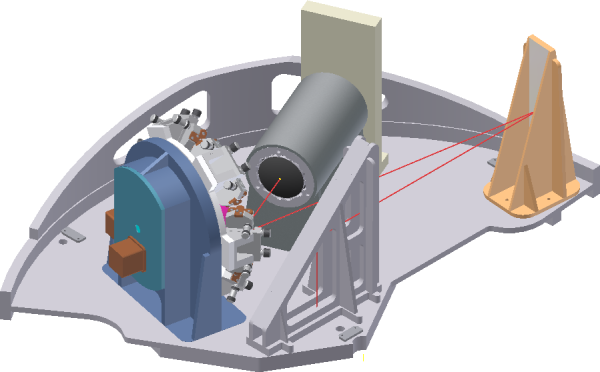
\includegraphics[width=0.65\textwidth]{kmos/kmos-spectrograph}
 \caption[The KMOS light path]{The light path for one of the three KMOS spectrograph demonstrated by the solid red line.
 The integral field unit entrance slit is located underneath the baseplate.
 The light path comes from the slit entrance and is redirected by the fold mirror toward the collimator (right, highlighted in yellow), where the light then is directed to the grating (left, housed in the blue filter wheel containing all 5 gratings) which disperses the light in camera barrel which finally focuses the light onto the detector (where the detector mount is in beige).
 \label{fig:kmoslight}}
\end{figure}

KMOS was designed with specific science goals which revolved around the case for spatially resolving the structure in galaxies across a large range of redshifts and environments~\citep{2006NewAR..50..370S} and,
as the most-efficient near-IR multi-object spectrograph in the southern hemisphere (and the only one on an 8-m telescope),
KMOS has gained significant attention from the scientific community.
Following successful commissioning runs KMOS underwent two science verification (SV) runs before being made available to the community for general observing in October 2013~\citep{2015IAUS..309...11S}.
Since then, KMOS has been used to study many different science goals and has already had an impact in the fields of some of its key science drivers~\citep{2016MNRAS.456.1195H,2016MNRAS.456.4533M}, as well as some intriguing results in other areas~\citep{2015A&A...584A...2F,2015MNRAS.453.3875P}.

In addition, KMOS has been exploited as a multi-object spectrograph to study the metallicities of star-forming galaxies using RSGs as cosmic abundance probes~\citep{2015ApJ...805..182G,2015ApJ...812..160L,2015ApJ...803...14P}.
% This programme is described in detail~\ref{ch:janal}.
This thesis makes extensive use of KMOS and would not be possible without this state-of-the-art instrument.


% section the_instrument (end)

\section{Production of Three-dimensional Data Cubes} % (fold)
\label{sec:3Ddata}

The nature of IFS is to obtain spatial and spectral information for each pixel on a detector.
The final data product is, therefore, a three dimensional data cube, which consists of two spatial and one spectral dimensions.
Therefore, the aim of the data reduction and calibration process is to create a regularly-sampled data cube from several raw detector images.

As mentioned, KMOS is arranged into three identical segments.
Each segment contains eight IFUs, which are arranged to project data onto a single detector.
Each IFU contains an advanced image slicer, which slices the field into 14 slices (see Figure~\ref{fig:image_slicer}), each of which contain 14 spatial pixels.
Therefore, each IFU produces 196 individual spectra and a single detector contains over 1500 spectra.
An example of a raw data product with KMOS is illustrated in Figure~\ref{fig:kmosdata} and highlights that each IFU contains 14 spectra each of width 14 pixels on the detector.
This figure demonstrates how the dispersed spectra are arranged on the detector.

\begin{figure}
 \centering
 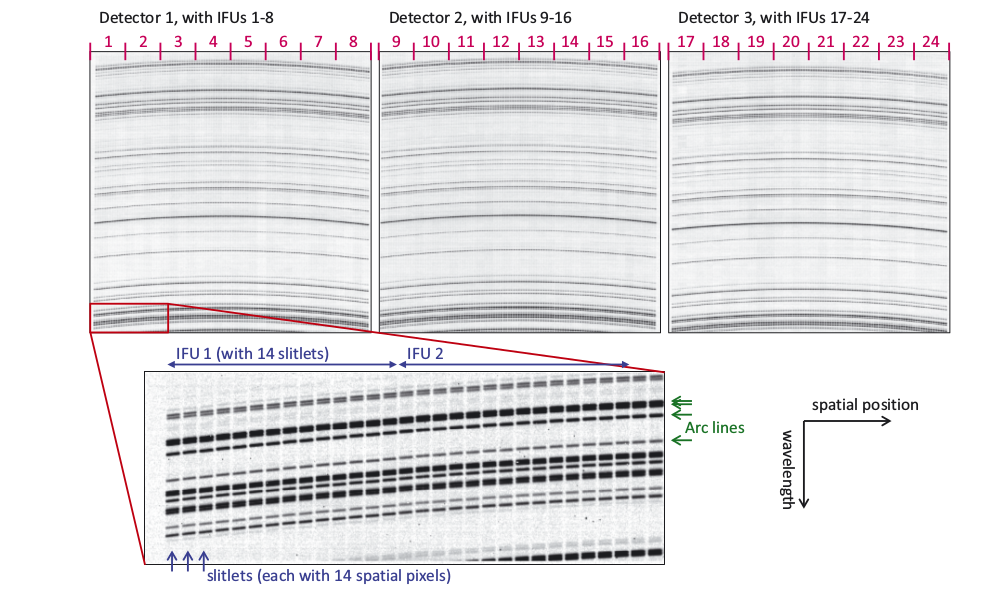
\includegraphics[width=0.65\textwidth]{kmos/kmos-data-Davies13}
 \caption[An example of KMOS raw data]{An example of a KMOS raw data product form, taken from~\citet{2013A&A...558A..56D}.
 This figure illustrates that, in one frame, light is dispersed onto one of three detectors.
 Each detector records light from eight IFUs,
 which is dispersed roughly in alignment with the $y$-axis on the detector.
 Each IFU contains 14 spectra with a width of 14 detector pixels and, therefore, the $x$-axis roughly corresponds to the spatial axis.
 \label{fig:kmosdata}}
\end{figure}

KMOS is designed so that, on the detector, the $x$- and $y$-axes roughly correspond to the spatial and spectral axes respectively.
However, on the detector there is no concept of spatial and spectral axes,
only information which can be calibrated and reconstructed into regularly sampled cubes containing spatial and spectral information.


\subsection{Calibration} % (fold)
\label{sub:calibration}

To calibrate KMOS data each value recorded by the detector must be assigned spatial and spectral information.
To do this one can use the projection of the light onto the detector, and the reliability of this projection, as a detailed diagnostic.
Slitlets are projected on the detector to $\pm$\,1\,$\mu$m
\citep[roughly 1/18$^{\rm th}$ of a pixel;][]{2013A&A...558A..56D} and
the mean slit-width across the detector is 13.6\,$\pm$\,0.1\,pixels,
where the error quoted here is the standard deviation of the mean from all slitlets.
This pattern is so stable that subtle imprints of the opto-mechanical design of the instrument can be seen in the patterns~\citep[see Fig. 2 of ][]{2013A&A...558A..56D}.

The main factor that affects this pattern is the temperature of the spectrograph.
As with any IR instrument, the detector must be cryogenically cooled to minimise the effects of photons from the thermal background promoting electrons into the conduction band of the semi-conducting diode of the detector, which are then confused with signal from the target.
For KMOS the detectors are cooled to $\le$80\,K.
In addition to the cooling of the detector, the optical bench -- which houses the spectrographs -- is also cooled to $\le$140\,K.
However, the temperature of the optical bench is not controlled and can therefore vary with the ambient temperature of the surroundings by several Kelvin.
This variation in temperature has a small, but significant, effect on the positions of the slitlet edges when compared in the calibration- and science-frames (described below).
The implications of this potential temperature variation of the optical bench is that during calibration frames, the temperature must be within $\pm$\,1\,K of the science frames.

To make use of the pattern of the slitlets on the detector, to calibrate the raw data, two types of calibration frames are obtained:

\begin{enumerate}
    \item Flat lamp calibrations use a halogen lamp with a white-light spectral appearance to fully illuminate each slitlet.
    These frames are used to calibrate the spatial positions of each detector pixel.

    \item Arc lamp calibrations use halogen lamps to create a spectrum containing many diagnostic spectral features, which are used to calibrate the wavelength of each detector pixel.
\end{enumerate}

These calibration frames are then compared with the science frames to construct a three dimensional data cube for each IFU.
An example of a reconstructed IFU is given in Figure~\ref{fig:kmosIFU}.
This figure is a snapshot of the reconstructed IFU at a particular wavelength.

\begin{figure}
 \centering
 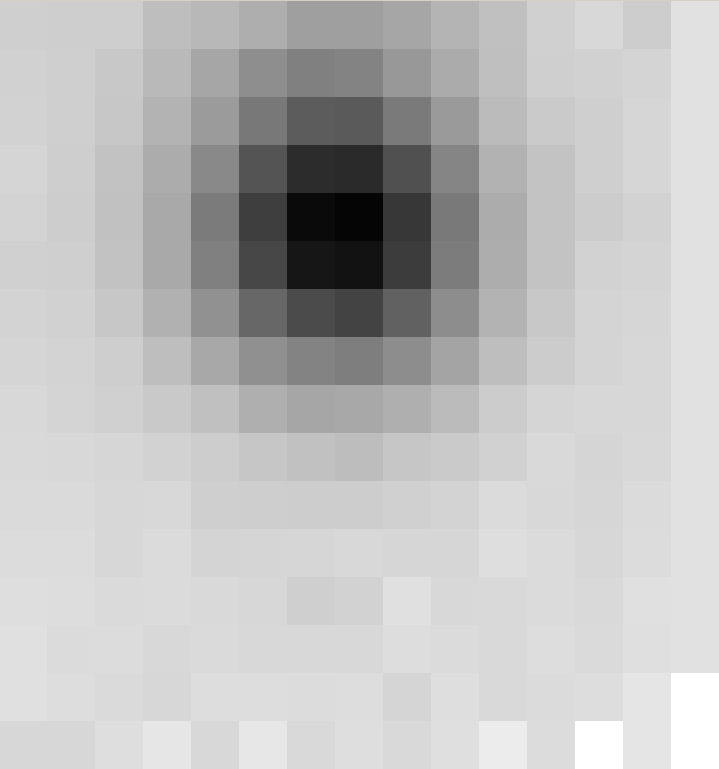
\includegraphics[width=0.65\textwidth]{kmos/ngc2100-ifu}
 \caption[An example of a reconstructed KMOS integral field unit]{An image of reconstructed KMOS integral field unit, demonstrating that each of the 14 slices of the field contains 14 pixels.
 This image is at a wavelength of 1.100\,$\mu$m.
 A spectrum is produced for each pixel and the current image is a snapshot at one particular spectral pixel.
 \label{fig:kmosIFU}}
\end{figure}

Calibration of the KMOS data can be split into three distinct processes:

\begin{enumerate}
    \item flatfielding,
    \item mapping data onto a regularly-sampled cube,
    \item correcting for atmospheric emission/absorption and instrument transmission.
\end{enumerate}

All of these processes are required to calibrate spectroscopic data in general, however, mapping the distortions of an instrument and transforming the data into a regularly sampled cube are instrument-dependent, and,
because of the complexity involved in arranging eight IFUs onto a detector, are the most important aspects in calibrating KMOS data.

Flatfielding is the process that corrects for the difference in response from detector pixels and is performed in a standard fashion using halogen lamps.
Flatfielding is also used to correct for variations in the illumination of the KMOS IFUs.
This is done directly using exposures from halogen lamps (lamp flats) and can be improved upon by using twilight sky to illuminate the detector (sky flats).
Using the twilight sky is, in general, preferred as the light path is identical to that of the science exposures.
However, observing in twilight conditions is extremely time dependent and in practice is difficult to undertake for an instrument as complex as KMOS.

To create a three dimensional data cube from KMOS raw data, a look-up table is created containing information relating each detector value with spatial and spectral locations.
This look-up table is implemented by creating three calibration files containing $x, y$ and $\lambda$ information for each pixel.
These calibration frames are created by making use of the repeatability of the pattern of the slitlets on the detector.
By fully illuminating the slitlets using the lamp-flat exposures the edge positions can be mapped from the calibration frames onto the science frames.
This provides the two spatial coordinates for each detector value.

To calibrate the wavelength of the each detector pixel one must illuminate the detector with a spectrum where the wavelength of each spectral feature is precisely known (i.e. the arc flats).
This is achieved with KMOS using a halogen lamp containing Neon and Argon where strong spectral features of known wavelengths cover the full detector range.
By identifying a few isolated spectral lines within these exposures, which are then traced across the length of the detector, a polynomial function is used to assign a wavelength solution to the detector.


At this stage, all the information needed to create the three dimensional data cube is available in three calibration frames.
This information is now used to transform the detector values onto a regularly sampled three dimensional data cube for each IFU.
It is necessary to perform multiple interpolations to the detector values, rather than simply rearranging these values, as -- in the frame of reference of the regularly sampled three dimensional data cube -- the detector values are irregularly sampled.
This is obvious from Figure~\ref{fig:kmosdata} which illustrates that the spectral and spatial axes are \textit{roughly} aligned with the $x$ and $y$ axes of the detector respectively.

As KMOS is a roughly three tonne instrument, the effects of flexure can be significant and are mainly caused by rotation of the instrument on the Nasmyth platform.
To account for this, calibration frames are taken at various rotator angles that are chosen to match the rotator angle of the science observations.
Using calibration frames at a more appropriate rotator angle can make a reasonable correction to the most serious sources of flexure.


There are, in principle, many different methods to create the data cube that affect the spectral and spatial resolution of the final data product.
The method that typically produces the highest quality data uses two (or three) one dimensional interpolations:
the so-called ``cubic spline interpolation'' routine in the pipeline.
This method makes use of two properties of the IFUs:

\begin{enumerate}
    \item each slitlet is a straight line when projected onto the sky,
    \item the spacing across each slitlet is fixed and uniform (as a result of the properties of the image slicers).
\end{enumerate}

By exploiting these properties this method is able to assign each detector pixel an $x$, $y$ and $\lambda$ value.
This is achieved by rearranging the detector values across each slitlet where no interpolation is necessary, using (ii).\footnotemark~Subsequently, a one dimensional cubic spline interpolation is performed along each slitlet, using i.
A final one dimensional cubic spline interpolation is performed in the spectral direction.
This method produces the best spectral resolution as well as giving highly consistent spatial resolution within each IFU.

\footnotetext{This is the case when the default sampling is used, when any other sampling is requested this step requires an additional interpolation performed using the cubic spline method.}


The final step in calibrating KMOS data is to take into account the effects of the Earth's atmosphere.
Observing from within the Earth's atmosphere affects the quality of the data in two different ways.
Intrinsically, when observing an astrophysical source through the Earth's atmosphere, each illuminated detector pixel contains a combination of source- and sky-photons.
Molecules and dust within the Earth's atmosphere scatter, absorb and emit light from the Earth and Moon which contaminates spectroscopic and photometric observations.
To account for this one typically attempts to observe a sky spectrum without any signal from the astrophysical source.
This usually takes the form of observing offset sky positions, where, between each target exposure, sky exposures are observed that are chosen to minimise contamination.
This results in an additional set of sky frames which are then used to calibrate the science frames using the same IFU in both science and sky exposures.
A simple example of the sky subtraction procedure is illustrated in Figure~\ref{fig:skysub}.
This figure shows that the signal from the sky is significantly larger than the signal from the object.
These sky frames are dealt with in the same manner as science frames in terms of calibration.
Typically, before the reconstruction of the three-dimensional data cubes however, the sky frame which is nearest in time to the science frame in question is subtracted.
% This correction can be improved upon by making small corrections to the sky cube using a sample of spatial pixels containing a smallest amount of target flux.

\begin{figure}
 \centering
 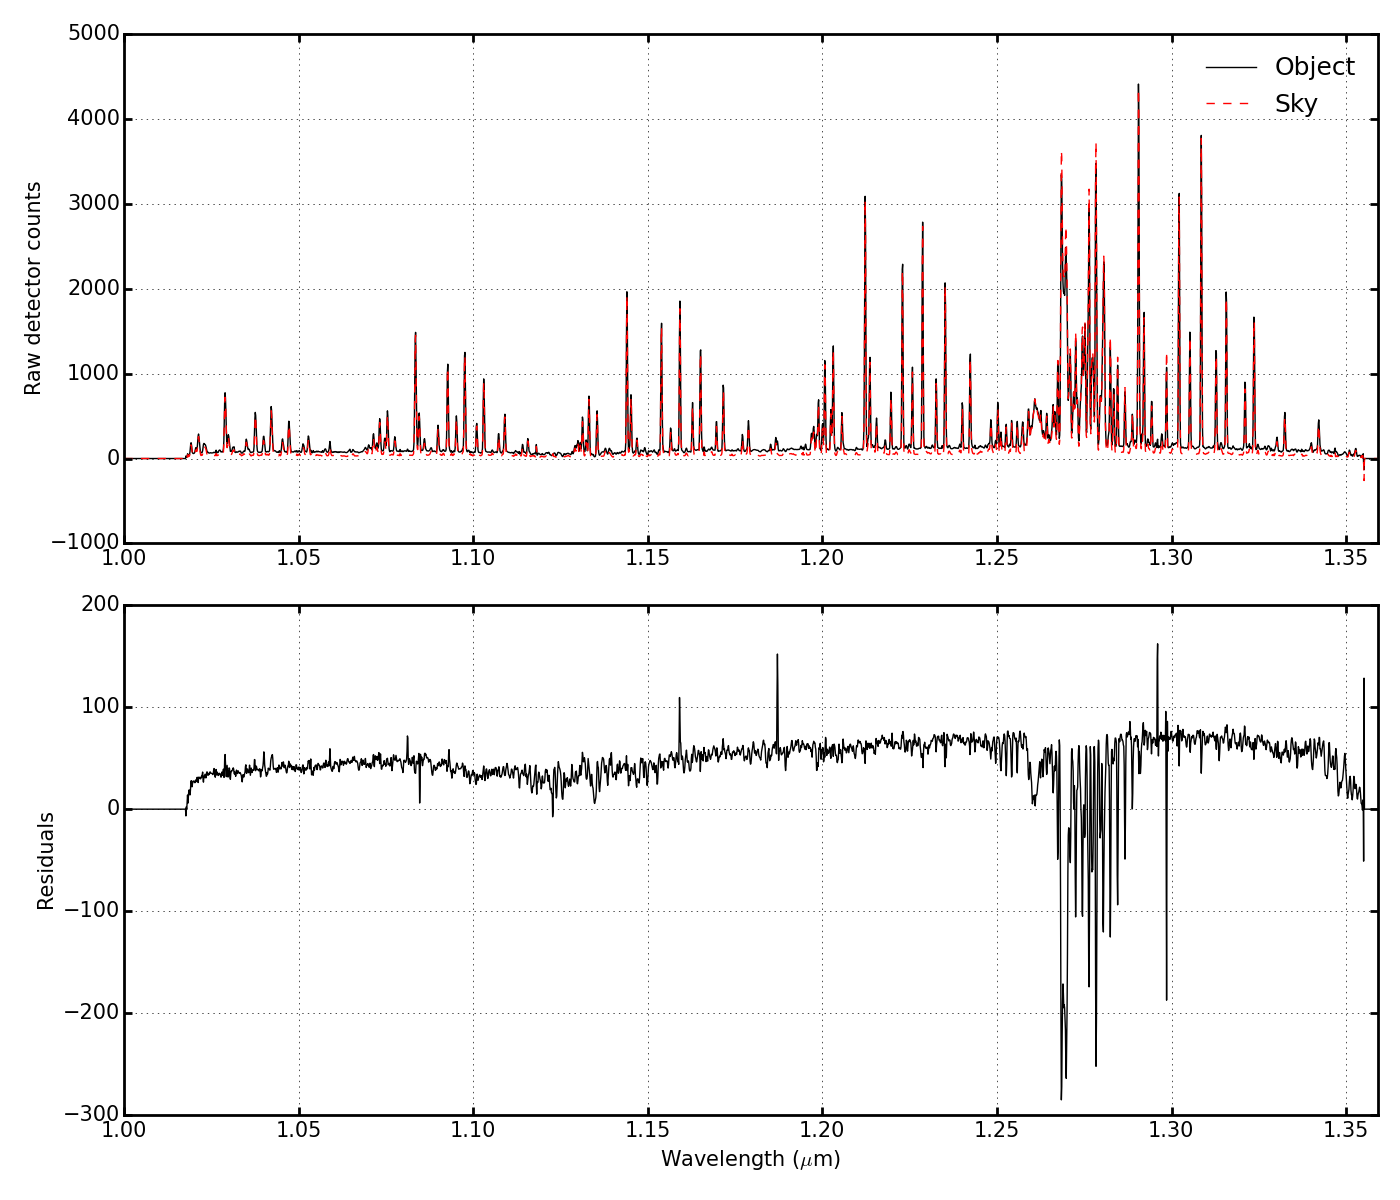
\includegraphics[width=0.85\textwidth]{kmos/NGC55-19-skysub_basic}
 \caption[An example of the sky subtraction procedure]{An example of the sky subtraction procedure. The top panel shows an object spectrum, in black, and an associated sky spectrum, in red.
 The bottom panel shows the sky subtracted spectrum by simply subtracting the two spectra in the top panel.
 Note the difference in scale between the two panels, illustrating that the signal from the sky is typically significantly larger than that from the object.
 \label{fig:skysub}}
\end{figure}

The second correction accounts for the absorption and re-emission of light from the science target by molecules within the Earth's atmosphere.
As the sophistication of this step is highly dependent upon the science case of the observations, for the general user this is implemented in a simplistic manner.
Typically, to perform this correction one observes an additional target of known spectral appearance: a telluric standard star.
This star is observed in each of the 24 KMOS IFUs in turn (or three IFUs depending upon the quality of the correction required) and the frames are calibrated using the same process as the science observations.

A spectrum is extracted from each IFU which is then divided by a model of the transmission of the atmosphere, the stellar features are then modelled with a simple Lorentzian function and removed.
This leaves a continuum spectrum of the star where the main features have been removed.
At this point the transmission model is then multiplied back into the spectrum and the shape of the spectrum is corrected with a blackbody spectrum, where the temperature is defined by the spectral type of the observed standard star.
Theoretically, these steps create a spectrum which contains only the light from the absorption of the Earth's atmosphere: the telluric spectrum.
The final target spectrum from an individual IFU is then divided by the telluric spectrum.

This is a simple overview of how one corrects for the effects of the Earth's atmosphere is KMOS observations.
For a more detailed discussion of how this can be improved see Chapter~\ref{ch:ngc2100} Section~\ref{sec:ngc2100obs} and Chapter~\ref{ch:ngc6822} Section~\ref{sec:ngc6822data_red}.

% subsection calibration (end)
% section data (end)

\section{Conclusions} % (fold)
\label{sec:kmosconc}

In this chapter, I have detailed the principles of spectroscopy and have outlined some of the key spectroscopic tools used to take astrophysical measurements, focusing on the diffraction grating and its uses in astronomy.
I have described IFS in detail and outlined some of the innovations that make this novel method possible.
I focused on using an advanced image slicer to perform IFS and outlined why this method is superior to other approaches.
This led onto a description of KMOS: the instrument used to obtain the spectroscopic data used in the subsequent chapters of this thesis.
In this section I detailed some of the key features that make this instrument unique and highlighted that KMOS has been applied to a range of science cases.
Finally, I described the data products from KMOS and detailed the process of calibration of the raw data.

% section conclusions (end)